% !TeX root = ../main.tex
\section{Введение}

\textbf{Цель работы:}
\begin{itemize}
    \item практическое освоение методов измерения основных линейных и нелинейных параметров транзисторных усилителей высокочастотного и СВЧ-диапазонов;
    \item приобретение навыков работы с цифровым анализатором спектра RIGOL DSA1030, высокочастотными генераторами сигналов, направленными ответвителями и сумматорами мощности;
    \item экспериментальное исследование амплитудно-частотной характеристики ($S_{21}$), обратного прохождения ($S_{12}$), коэффициента шума ($K_{\text{ш}}$), точки децибельной компрессии ($P_{1\text{dB}}$) и продуктов интермодуляции 3-го порядка ($IP_3$).
\end{itemize}

\textbf{Используемое оборудование и принадлежности:}
\begin{itemize}
    \item Цифровой анализатор спектра RIGOL DSA1030 (диапазон частот от 9~кГц до 3~ГГц);
    \item Генераторы высокочастотных гармонических сигналов Advantex SG8;
    \item Лабораторный регулируемый источник постоянного напряжения питания усилителя;
    \item Набор согласованных коаксиальных аттенюаторов фиксированного ослабления (6~дБ, 10~дБ, 20~дБ, 40~дБ);
    \item Делитель/сумматор мощности (Power Splitter/Combiner 1:2);
    \item Направленный ответвитель (Directional Coupler);
    \item Комплект калиброванных соединительных коаксиальных кабелей с разъемами SMA и переходные адаптеры $\text{SMA}(f)\text{--}\text{SMA}(f)$.
\end{itemize}

\section{Измерение коэффициента усиления ($S_{21}$) и коэффициента обратной развязки ($S_{12}$)}

Результаты измерений мощности и рассчитанные значения волновых коэффициентов передачи приведены в таблице~\ref{tab:s_params}.

\begin{table}[H]
\centering
\caption{Экспериментальные данные и результаты расчета параметров $S_{21}$ и $S_{12}$}
\label{tab:s_params}
\small
\begin{tabular}{|c|c|c|c|c|c|}
\hline
$f$, МГц & $P_{2\text{cal}}$, дБм & $P_{1\text{amp}}$, дБм & $P_{\text{rev}}$, дБм & $S_{21}$, дБ & $S_{12}$, дБ \\
\hline
10   & -47.00 & -25.00 & -68.00 & 22.00 & -21.00 \\
100  & -45.00 & -18.00 & -60.00 & 27.00 & -15.00 \\
200  & -44.00 & -16.00 & -58.00 & 28.00 & -14.00 \\
500  & -40.10 & -16.38 & -49.00 & 23.72 & -8.90  \\
700  & -41.20 & -16.95 & -48.65 & 24.25 & -7.45  \\
900  & -39.10 & -17.66 & -48.33 & 21.44 & -9.23  \\
1100 & -39.06 & -17.54 & -47.90 & 21.52 & -8.84  \\
1300 & -40.20 & -19.78 & -47.86 & 20.42 & -7.66  \\
1500 & -38.42 & -19.90 & -46.90 & 18.52 & -8.48  \\
1700 & -38.00 & -21.80 & -46.70 & 16.20 & -8.70  \\
1900 & -39.00 & -21.76 & -45.00 & 17.24 & -6.00  \\
2100 & -39.43 & -22.15 & -44.70 & 17.28 & -5.27  \\
2300 & -39.59 & -23.00 & -44.33 & 16.59 & -4.74  \\
2500 & -37.90 & -22.55 & -43.00 & 15.35 & -5.10  \\
2700 & -38.00 & -23.20 & -42.00 & 14.80 & -4.00  \\
2900 & -37.30 & -22.99 & -40.47 & 14.31 & -3.17  \\
\hline
\end{tabular}
\end{table}

На основе полученных данных построены графики амплитудно-частотной характеристики $S_{21}(f)$ (рис.~\ref{fig:s21}) и коэффициента обратного прохождения $S_{12}(f)$ (рис.~\ref{fig:s12}).

\begin{figure}[H]
    \centering
    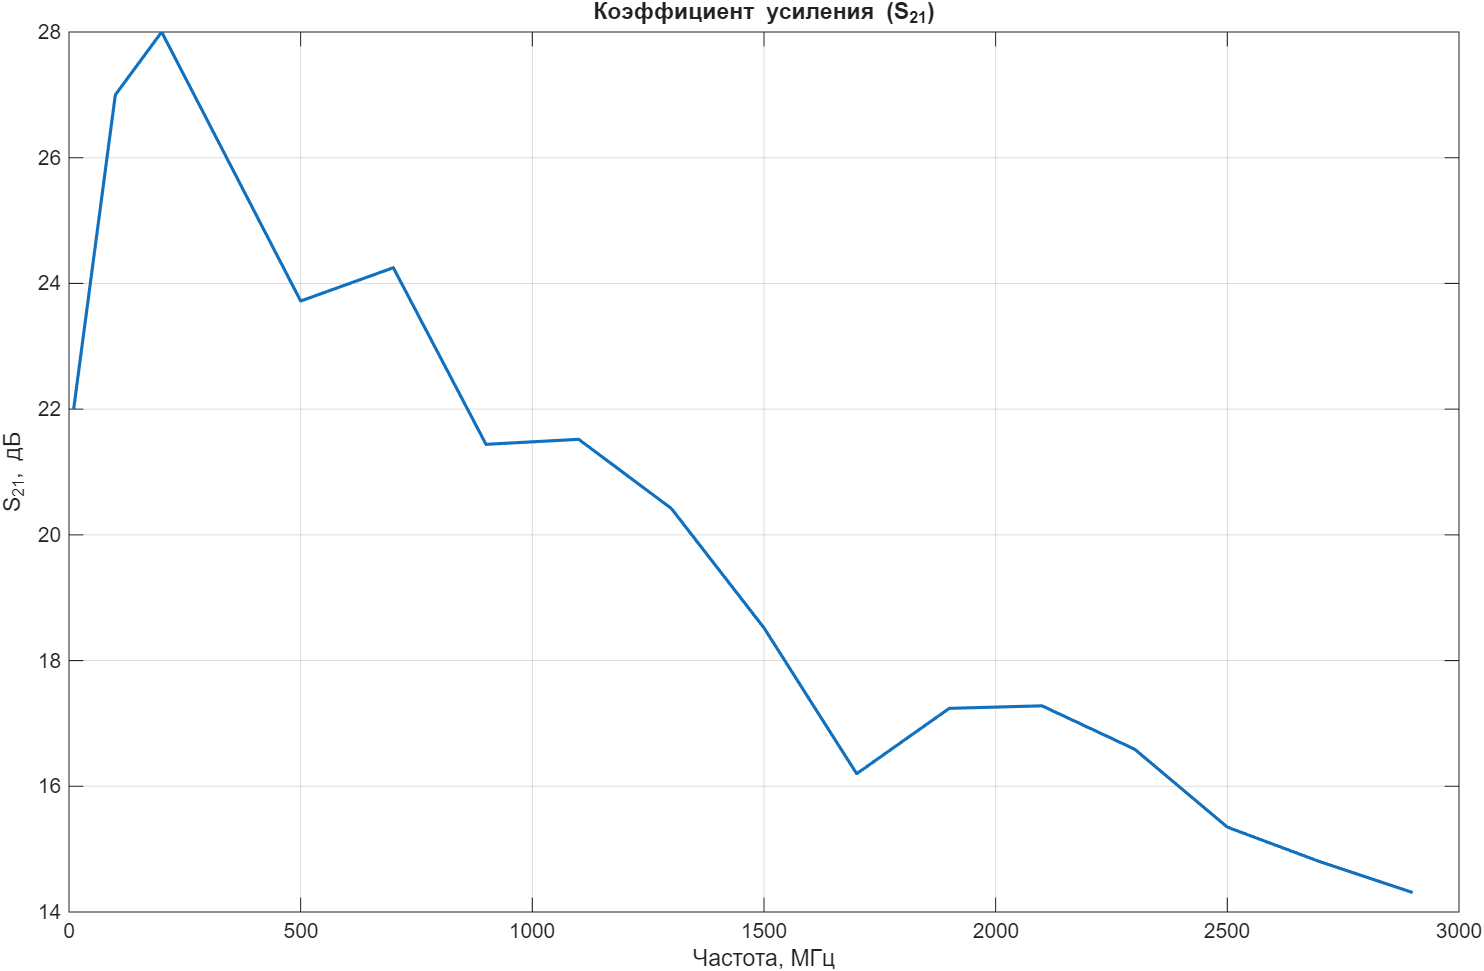
\includegraphics[width=0.88\textwidth]{ачх.png}
    \caption{Амплитудно-частотная характеристика усилителя (коэффициент усиления $S_{21}$ от частоты)}
    \label{fig:s21}
\end{figure}

\begin{figure}[H]
    \centering
    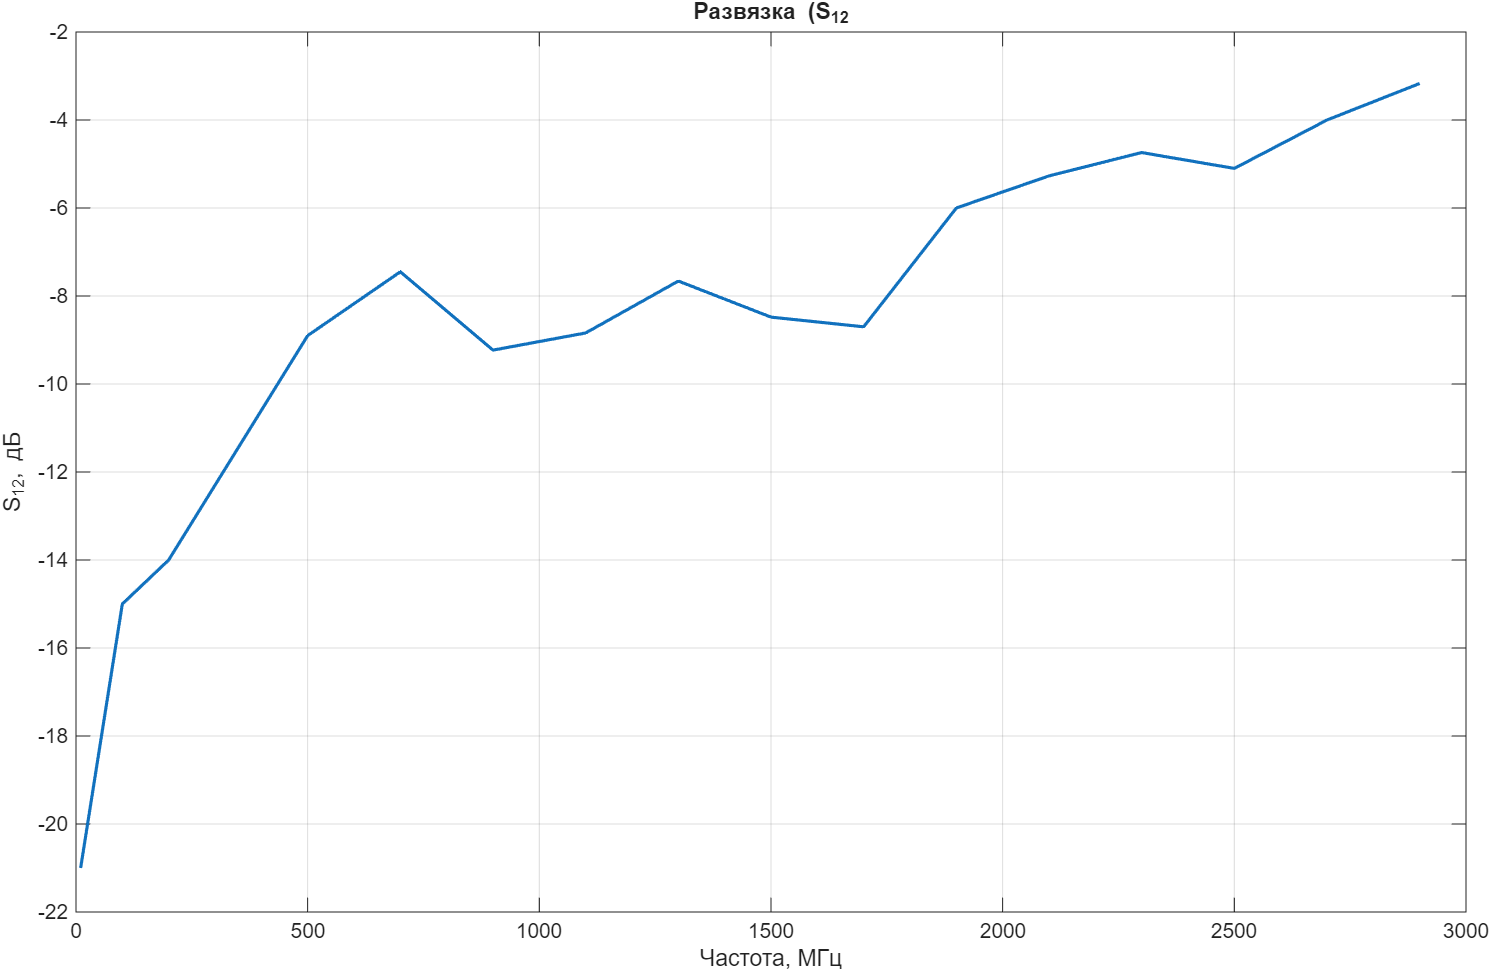
\includegraphics[width=0.88\textwidth]{развязка.png}
    \caption{Зависимость коэффициента обратной передачи ($S_{12}$) усилителя от частоты}
    \label{fig:s12}
\end{figure}

\subsection{Анализ результатов и выводы}

\begin{enumerate}
    \item \textbf{Коэффициент усиления ($S_{21}$):} Исследуемый усилитель обеспечивает максимальный коэффициент усиления в области частот 100--200~МГц ($S_{21} \approx 27\text{--}28\text{ дБ}$). В рабочем диапазоне от 500~МГц до 1300~МГц коэффициент усиления плавно снижается с 23.7~дБ до 20.4~дБ, а на частотах свыше 1.5~ГГц спад усилительных свойств усиливается вплоть до 14.3~дБ на частоте 2900~МГц. Уменьшение коэффициента усиления с ростом частоты объясняется влиянием паразитных барьерных и диффузионных емкостей транзисторов и падением крутизны усилительного каскада.
    \item \textbf{Обратная развязка ($S_{12}$):} На низких частотах (10--200~МГц) каскад демонстрирует высокую развязку (от $-21\text{ дБ}$ до $-14\text{ дБ}$). Однако с увеличением частоты модуль коэффициента обратной передачи $S_{12}$ возрастает, достигая $-3.17\text{ дБ}$ на частоте 2900~МГц. Это свидетельствует об ухудшении изолирующих свойств транзистора на СВЧ из-за емкостной связи между выходом и входом через проходную емкость коллектор-база (сток-затвор).
    \item \textbf{Роль калибровочных измерений:} Проведение предварительной калибровки тракта позволило скомпенсировать частотную зависимость затухания кабелей и внешнего аттенюатора (изменение $P_{2\text{cal}}$ от $-47.0\text{ дБм}$ до $-37.3\text{ дБм}$), исключив систематическую аппаратную погрешность из итоговых значений $S$-параметров.
\end{enumerate}